\section{Captive Portal - Proof of Concept}
\label{section:realisation:captive_portal}
\subsection{Lastenheft}
Nach dem Treffen mit PulseShift am 08.03.2018 wurde ein Lastenheft mit den folgenden Punkten ausgearbeitet:
\begin{itemize}
\item Es soll ein Captive Portal innerhalb eines WLAN Netzwerks eingerichtet werden, das die Nutzer optional zu einer Umfrage weiterleiten kann.
\item Es sollen mehrere Hardwarelösungen mit Captive Portal Funktionalität, wie ein Raspberry Pi, ein Router oder ein Accesspoint, untersucht werden. 
\item Anschließend soll das Captive Portal durch genau eine der untersuchten Hardwarelösungen realisiert werden.
\item Die dabei benötigte Hardware soll unter Absprache mit Pulseshift von Pulseshift organisiert werden.
\item Der Nutzer, der ein Endgerät mit dem erzeugten WLAN Netzwerk verbindet, soll über die Möglichkeit zur Teilnahme an einer Umfrage informiert, jedoch nicht gezwungen werden.
\item Durch einen Redirect soll der Nutzer direkt zu einer Umfrageseite gelangen, die die Fragebögen von Pulseshift beinhaltet.
\item Die Fragebögen von Pulseshift sollen entweder lokal auf der Hardwarelösung gespeichert sein oder über das Internet direkt angesteuert werden.
\end{itemize}

\subsection{Pflichtenheft}
Anhand des zuvor erarbeiteten Lastenhefts wurde anschließend ein Pflichtenheft mit folgendem Inhalt erstellt:
\begin{itemize}
\item Es werden Hardwarelösungen mit Captive Portal Funktionalität untersucht.
\item Dabei werden Router, Accesspoints und Rasbperry Pis genauer behandelt.
\item Die Anwendungsmöglichkeiten, Vor- \& Nachteile der einzelnen Komponenten wird erarbeitet.
\item Als weiteres Auswahlkriterium wird überprüft, ob eine entsprechende Lösung unabhängig vom Hersteller der Hardware erfolgen kann.
\item Unter Absprache mit Pulseshift wird eine entsprechende Hardwarelösung von Pulseshift bereitgestellt.
\item Die gegebene Hardwarelösung wird ein WLAN Netzwerk erzeugen, indem sich Nutzer, die sich in unmittelbarer Nähe befinden, mit ihren Endgeräten anmelden können.
\item Nach dem Anmelden erfolgt eine Weiterleitung zur lokal gehosteten oder über das Internet erreichbaren Umfrageseite.
\end{itemize}



\subsection{EPK: Ablauf der Anwendung}

Die in \ref{fig:captive_epk1} dargestellte EPK zeigt den Ablauf der Captive Portal Funktionalität ohne Internet, wie er etwa bei Gesamtveranstaltungen genutzt werden kann. Nach der Verbindung des Nutzers mit dem WLAN erscheint automatisch ein Pop-up mit der Umfrageseite. Vorteil hierbei ist, dass keine URL eingegeben werden muss und die Endgeräte keinen Internetzugang benötigen. Theoretisch kann diese Lösung auch dauerhaft in der Kantine aufgestellt werden, da jedoch kein Internetzugang besteht, ist der Anreiz gering, sich mit dem WLAN zu verbinden.
\newline
\begin{figure}[H]
\centering
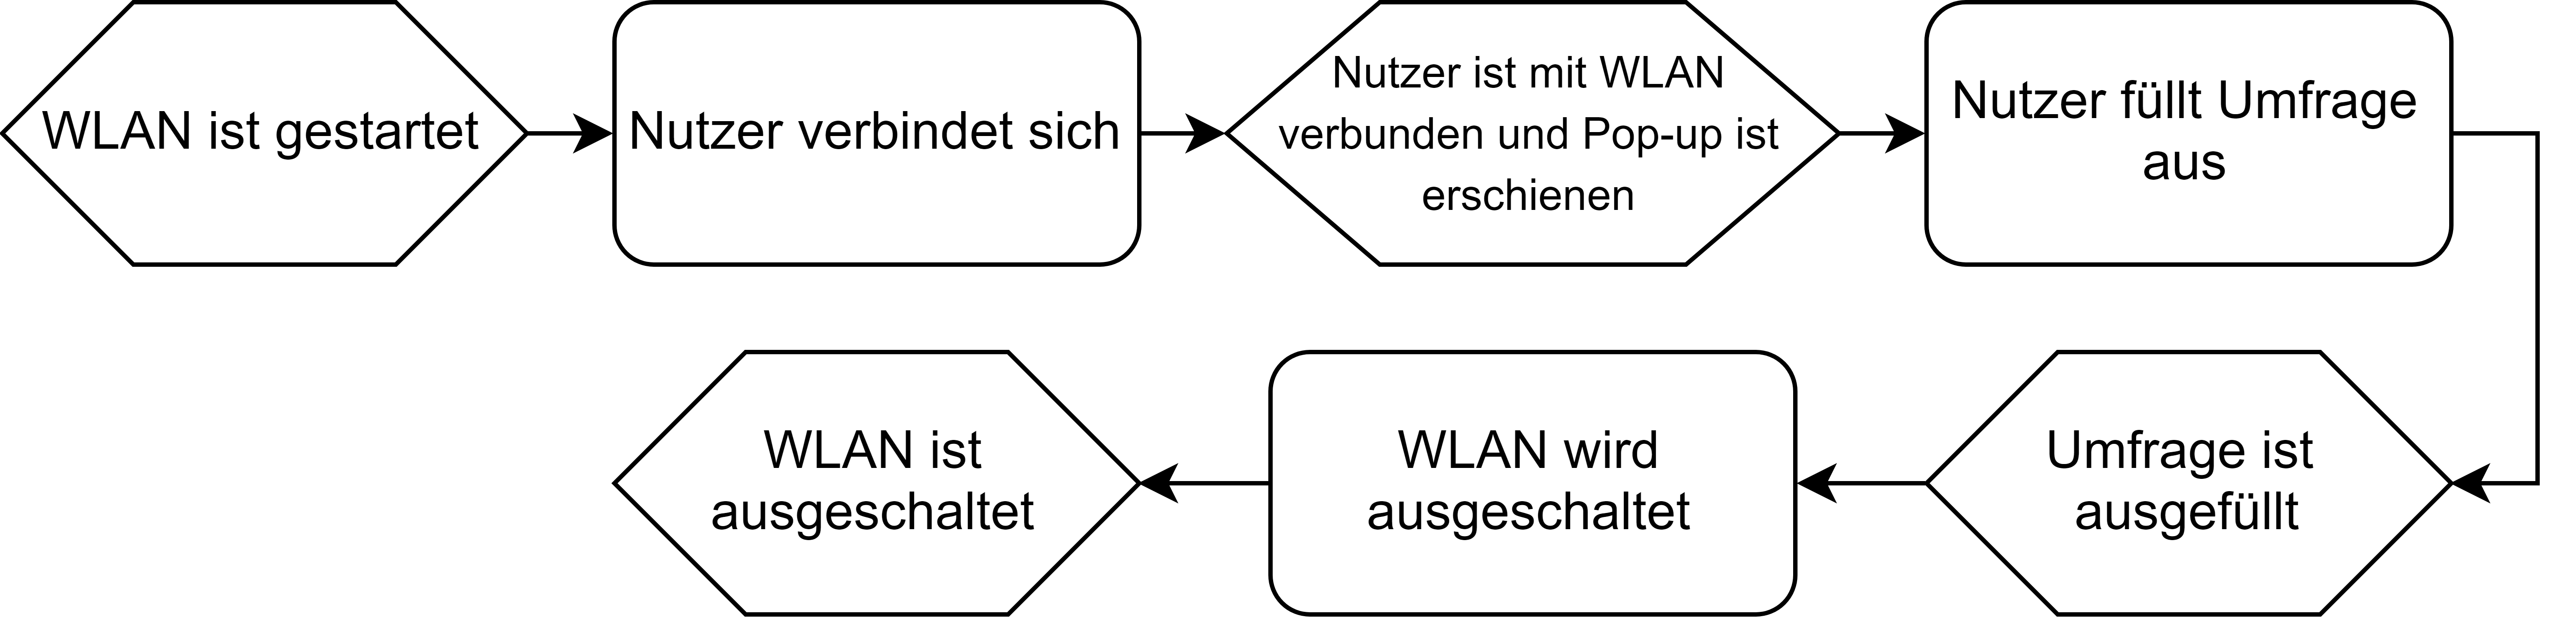
\includegraphics[width=0.9\textwidth]{images/captiveportal_EPK1}
\caption[EPK zum Ablauf ohne Internetzugang]{EPK zum Ablauf ohne Internetzugang}
\label{fig:captive_epk1}
\end{figure}


Die in \ref{fig:captive_epk2} dargestellte EPK zeigt die Verwendung eines Captive Portals mit Internetzugang. Diese Lösung könnte bei einem längerfristigen Einsatz Anwendung finden und während des Umfragezeitraums etwa in der Kantine vor den Internetzugang geschaltet werden. Nachdem sich der Nutzer mit dem WLAN verbunden hat, erscheint auch hier der Pop-up mit der Umfrageseite. Da der Nutzer nicht gezwungen werden darf, diese auszufüllen, kann sie durch einen \textit{Überspringen}-Button übersprungen werden und der Nutzer gelangt direkt ins Internet. Alternativ füllt der Nutzer die Umfrage aus und erhält im Anschluss den Zugang ins Internet. Soll die Umfrage erneut durchgeführt werden, kann der Nutzer - etwa durch einen Timeout - vom WLAN abgemeldet werden und er erhält bei der nächsten Verbindung erneut das Pop-up mit der Umfrageseite und anderen Fragen.

\begin{figure}[H]
\centering
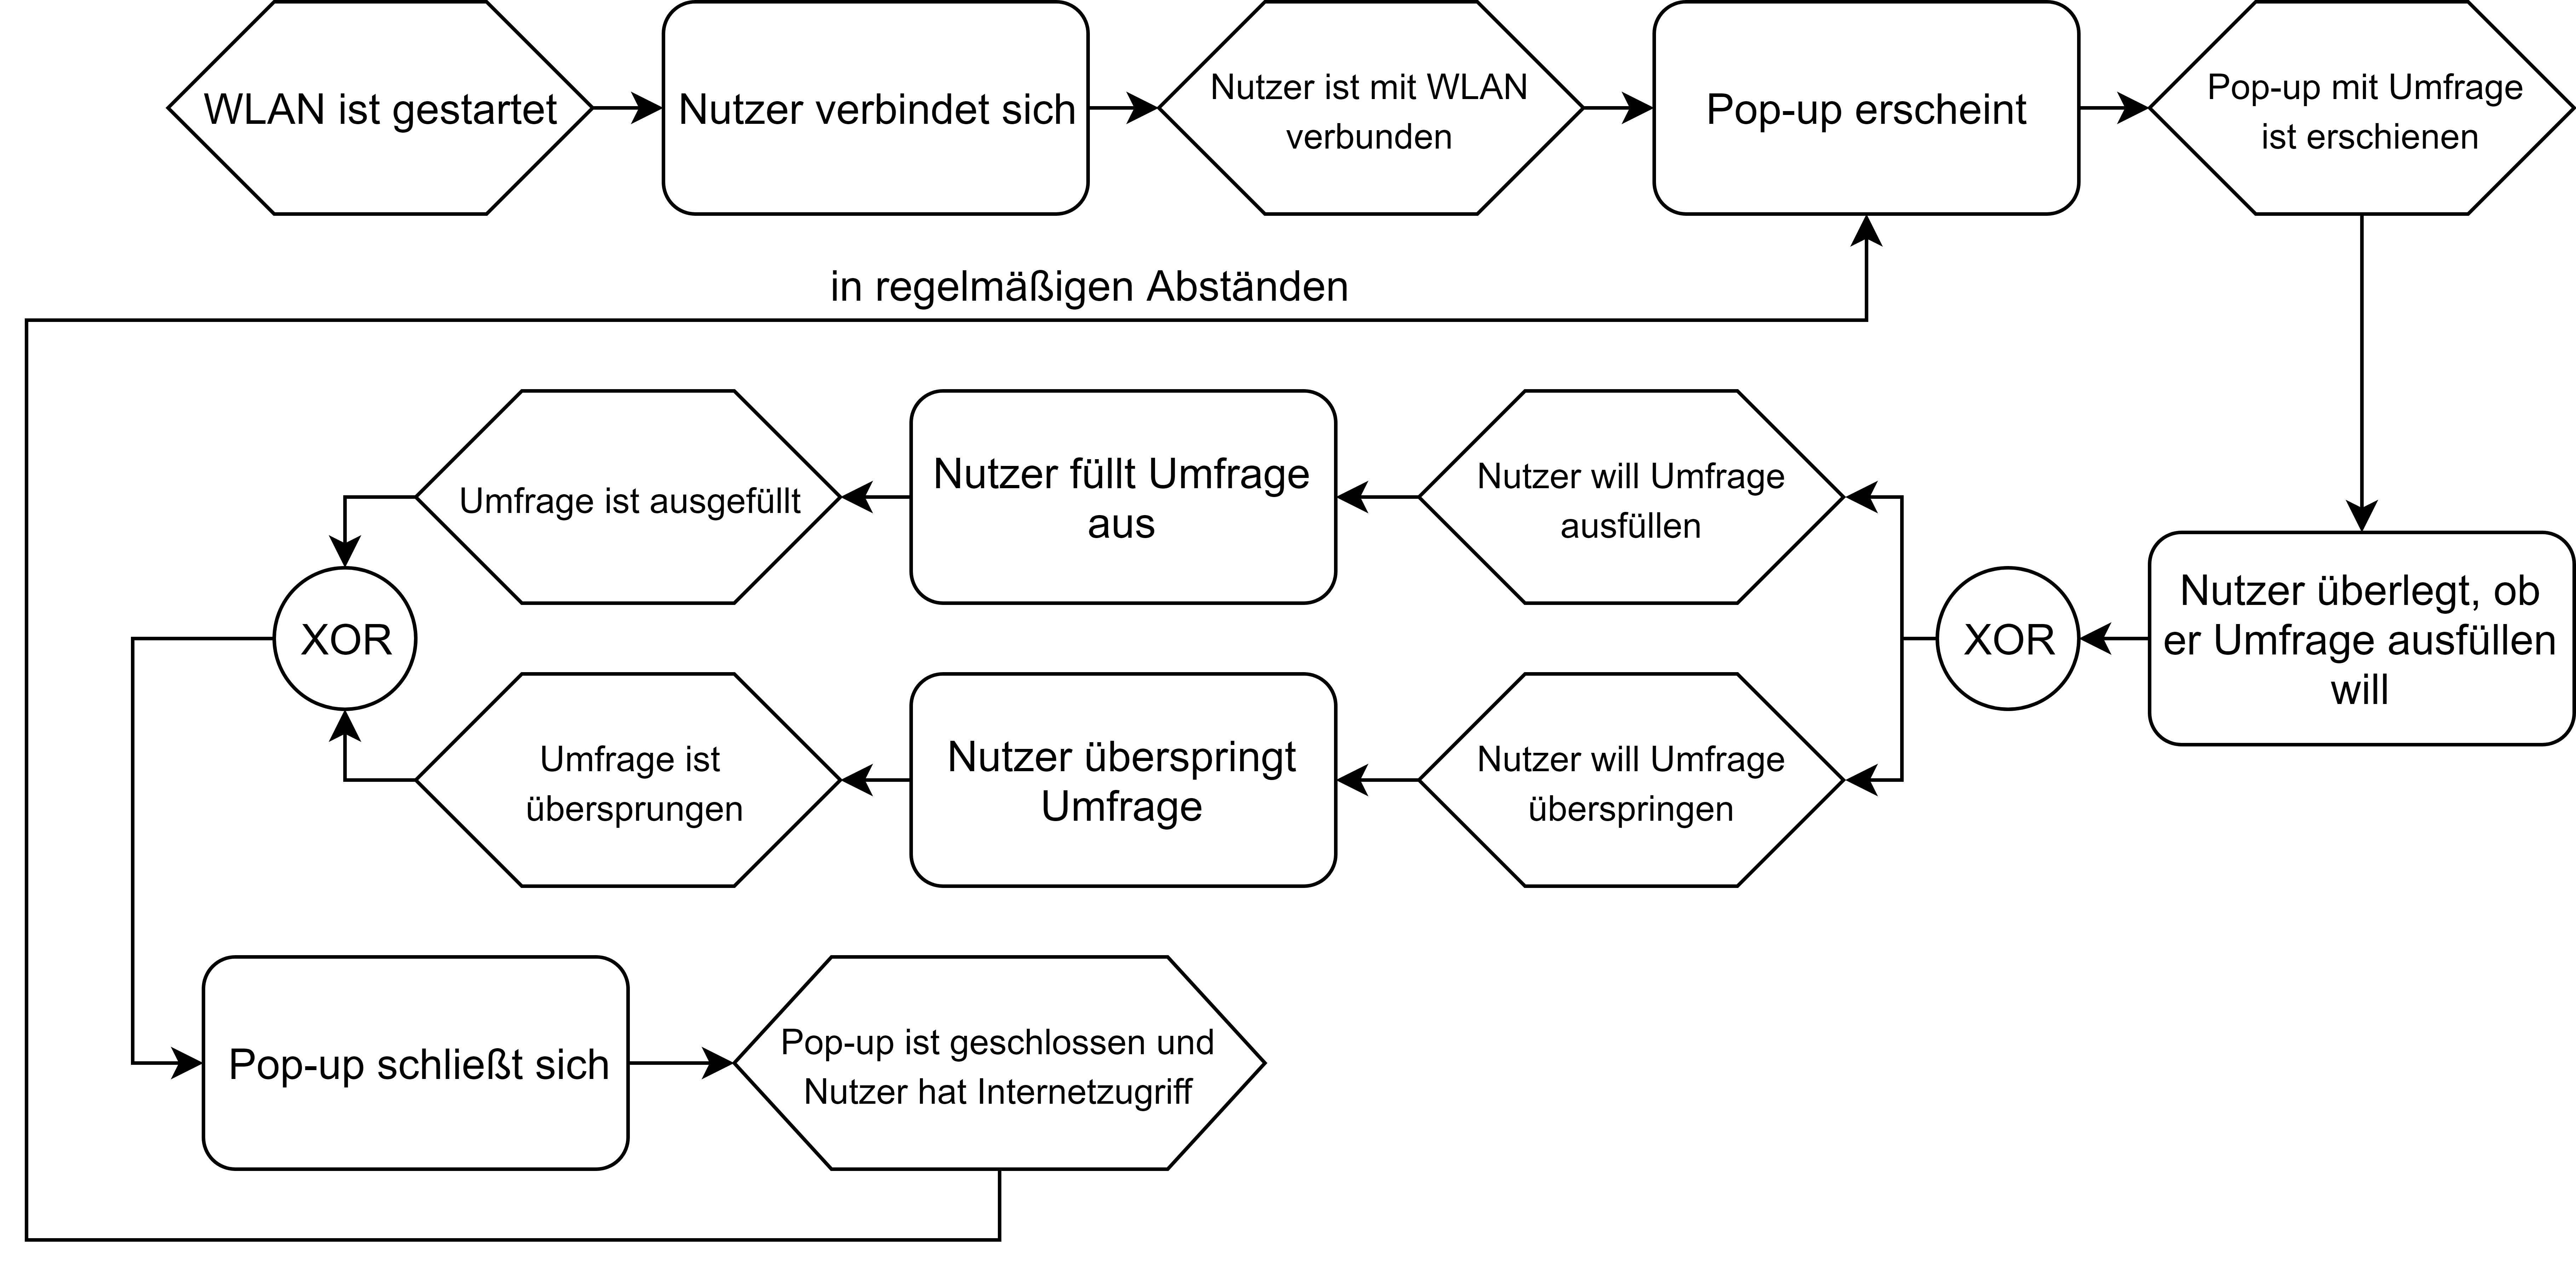
\includegraphics[width=0.9\textwidth]{images/captiveportal_EPK2}
\caption[EPK zum Ablauf mit Internetzugang]{EPK zum Ablauf mit Internetzugang}
\label{fig:captive_epk2}
\end{figure}

 
\subsection{Architektur}
\subsubsection{Verwendung eines Raspberry Pi}
\subsubsection*{Initiale Einrichtung und verwendete Hardware}
Der Raspberry Pi soll die Funktionalität eines Captive Portals für Umfragen veranschaulichen. Grundsätzlich benötigt wird hierfür:
\begin{itemize}
\item Raspberry Pi 3
\item Stromkabel
\item SD Karte
\end{itemize}

Da der Raspberry Pi 3 bereits einen WLAN-Empfänger eingebaut hat, wird kein zusätzlicher WLAN-USB-Empfänger benötigt. Zunächst muss das Betriebssystem Raspbian Stretch auf dem Raspberry Pi  installiert werden. Hierfür kann beispielsweise das Installationsprogramm \textit{NOOBS} genutzt werden, das über einen Computer auf die SD Karte gespielt wird. Anschließend erfolgt die Installation und die Aktualisierung des Betriebssystems durch \textit{apt-get update} und \textit{apt-get upgrade}.

\subsubsection*{Anleitung 1 - Captive Portal ohne Internet}
Um das Captive Portal einzurichten, wird zunächst der Ansatz ohne Internetverbindung, also mit einer lokal gehosteten Webseite, gewählt. Diese eignet sich insbesondere für die Verwendung bei Gesamtveranstaltungen, bei denen die Umfrage einmalig durchgeführt wird. Hierfür wird der unter \textit{https://brennanhm.ca/knowledgebase/2016 /10/raspberry-pi-access-point-and-captive-portal-without-internet/} zu findenden Anleitung gefolgt. Um diese umzusetzen, müssen auf dem Raspberry Pi die Pakete \textit{hostapd} und \textit{dnsmasq} installiert werden.

Das Paket \textit{hostapd} ermöglicht es, dass der WLAN-Empfänger als Access Point dienen kann, also Verbindungen von anderen Endgeräten annimmt. Bei dem Paket \textit{dnsmasq} handelt es sich um einen einfach zu konfigurierenden DNS- und DHCP-Server. Für beide Pakete müssen anschließend weitere Konfigurationen durchgeführt werden.

Das letzte Paket \textit{nginx} bietet einen Webserver, der für das lokale Hosting der Umfrage-Seite genutzt wird. Die in der Anleitung vorgeschlagene \textit{nginx}-Konfiguration wird um ein von der Umfrageseite benötigtes rewrite-Statement für den Pfad /feedback/ ergänzt. In dem Block für den /generate\_204 Pfad können URL-Parameter mitzurückgegeben werden. Diese werden auch auf Android und auf Windows Endgeräten genutzt, bei iOS hingegen funktioniert dies nicht. Aus diesem Grund wurden diese URL-Parameter, nach unterschiedlichen Versuchen, nginx richtig zu konfigurieren, direkt in der JavaScript-Datei der Umfrage-Webseite festgelegt. Der Nutzer wird ebenfalls auf die Umfrageseite weitergeleitet, wenn er eine beliebige URL in seinen Browser eingibt.

Das Captive Portal des Raspberry Pi funktioniert mit dieser Anleitung problemlos auf Windows-Computern, iOS-Endgeräten und den meisten Android-Engeräten. Lediglich bei Samsung-Smartphones öffnet sich der Pop-up zum Anmelden am WLAN nicht. Der Grund hierfür ist nicht klar, könnte jedoch möglicherweise durch eine andere dnsmasq- oder nginx-Konfiguration behoben werden.

Die automatische Einrichtung des Raspberry Pi wird durch ein selbst erstellten Shell Skript ermöglicht, dass die Schritte in der Anleitung hintereinander durchführt. Voraussetzung ist ein neu aufgesetzter Raspberry Pi 3 mit WLAN-Interface wlan0. Der Name des WLAN-Netzwerks wird als Argument \textit{sudo bash setup.sh Name\_des\_WLANs} übergeben, die Webseite muss anschließend in den Ordner /usr/share/nginx/html/host kopiert werden.

\subsubsection*{Anleitung 2 - Captive Portal mit Internet}
Eine zweite Anleitung ermöglicht es, den Raspberry Pi als WLAN-Access Point mit Captive Portal für einen Internetzugang zu nutzen, was für den längerfristigen Einsatz - etwa in einer Kantine - geeignet wäre. Hierfür werden die Anleitungen 2a unter \textit{https://pimylifeup.com/raspberry-pi-wireless-access-point/} für die Einrichtung des Access Points und 2b unter \textit{https://pimylifeup.com/raspberry-pi-captive-portal/} für die Captive Portal Funktionalität genutzt.

Für die Einrichtung des Access Points werden erneut die Pakete \textit{hostapd} und \textit{dnsmasq} genutzt. Zusätzlich werden die IP-Tabellen verändert und diese Veränderungen und ein Neustart von \textit{hostapd} und \textit{dnsmasq} in die rc.local Datei geschrieben, damit diese bei jedem Neustart umgesetzt werden. Dies hat jedoch bei dem Austesten der Anleitung nicht funktioniert, sodass ein \textit{sleep 10} Befehl der rc.local Datei hinzugefügt werden musste.

Im zweiten Schritt wird für den Access Point die Captive Portal Funktionalität hinzugefügt. Hierfür wird die Software \textit{nodogsplash} auf dem Raspberry Pi installiert. Diese hostet lokal die Captive Portal Seite in dem Verzeichnis \textit{/etc/nodogsplash/htdocs/splash.html}. Auf der Captive Portal Seite kann ein Formular abgeschickt werden, mit dem der Nutzer authentifiziert wird und mit dem er Zugriff auf das Internet erhält. Dieses kann zum Überspringen der Umfrage direkt oder erst nach dem Ausfüllen der Anfrage abgeschickt werden. Hierfür müsste der Umfrage-Webapp ein \textit{Überspringen}-Button und ein \textit{Umfrage abschließen}-Button hinzugefügt werden, durch die das Formular abgeschickt wird. In der nodogsplash.conf Datei können weitere Konfigurationen vorgenommen werden, insbesondere auch der Internetzugriff für nicht-authentifizierte Nutzer erlaubt werden, sodass auf der Captive Portal Seite Inhalte aus dem Internet angezeigt werden.

Diese Lösung funktioniert auf allen Endgeräten, insbesondere auch auf denen von Samsung. Liegt kein Internet vor, funktioniert das Captive Portal jedoch nicht. Hierfür muss in der dnsmasq.conf Konfigurationsdatei \textit{address=/\#/IP\_des\_Raspberry} zur Auflösung aller Domainnamen auf den Raspberry Pi hinzugefügt werden. Ist dies erfolgt, funktioniert das automatische Pop-up bei Samsung Smartphones jedoch nicht mehr.

Auch für diese Anleitungen wurden Shell Skripte umgesetzt. Diese können mit \textit{sudo bash setup2a.sh Name\_des\_WLANs Passwort\_des\_WLANs} und \textit{sudo bash setup2b.sh} ausgeführt werden.

\subsubsection*{Weiteres Vorgehen}
Die Umsetzung des Captive Portals mithilfe des Raspberry Pi dient in erster Linie zur Veranschaulichung der Möglichkeit, die Umfrage in dieser Form umzusetzen. Sollte eine der Lösungen des Raspberry Pi tatsächlich in einem produktiven Umfeld genutzt werden, sind folgende Aspekte zu beachten:
\begin{itemize}
\item Es sollte ein externer WLAN-Empfänger genutzt werden, da der in dem Raspberry Pi eingebaute Empfänger vermutlich eine zu geringe Signalstärke hat. In diesem Fall müssten die Konfigurationen entsprechend angepasst werden. Gleichzeitig muss überprüft werden, wie viel Verbindungen gleichzeitig unterstützt werden können.
\item Das Problem der automatischen Pop-ups bei Samsung Handys muss behoben werden; es liegt womöglich an der DNS-Auflösung oder der zurückgegebenen Status-Codes.
\item Die Anleitungen müssen vertieft auf die Aspekte Sicherheit und Performance überprüft und möglicherweise auch eine SSL-Verschlüsselung eingerichtet werden. Die Lösungen sollten in der bestehenden Form noch nicht produktiv genutzt werden, da Sicherheitsrisiken bestehen, die insbesondere bei der zweiten, längerfristigen Lösung mit Internetzugang gefährlich sind.

\end{itemize}

\subsubsection{Alternative Ansätze}
Neben der Verwendung des Raspberry Pi gibt es verschiedene Hardware- und Softwarelösungen, die ebenfalls die Captive Portal Funktionalität bieten. Vorteil von diesen ist, dass es sich in der Regel bereits um fertig konfigurierte und funktionierende Lösungen handelt; Nachteil ist hingegen, dass häufig wenig Konfigurationen möglich sind.

Bietet ein Unternehmen seinen Mitarbeitern einen WLAN-Internetzugang an, so wird dieser meist über zentral verwaltete Access Points realisiert. Hier besteht die Möglichkeit, dass der Access Point bereits eine Captive Portal Funktionalität besitzt. Die meiste vorinstallierte Software besitzt jedoch nur die Möglichkeit, eine einfache Webseite zum Akzeptieren der Nutzungsbedingungen anzuzeigen, sodass die eigene Umfrageseite nicht einfach eingebunden werden kann (z.B. nur als Redirect nach dem Akzeptieren der Nutzungsbedingungen). Aus diesem Grund ist es unwahrscheinlich, dass die Umfrageseite als Captive Portal direkt in der Access Point Software eines Unternehmens aktiviert werden kann.

Eine andere Lösung ist es, beispielsweise die Firewall- und Router-Software pfSense vor die Access Points oder bei Gesamtveranstaltungen vor einen eigenen Access Point zu schalten. Diese ermöglicht ebenfalls die Captive Portal Funktionalität. Der Einsatz ist jedoch in einem Firmennetzwerk er unwahrscheinlich, da ein größerer Eingriff in die Ntzwerkinfrastruktur erforderlich ist.

Als Alternative könnte auch das Betriebssystem eines kompatiblen Routers durch das auf Linux basierende, weit verbreitete Betriebssystem OpenWRT überschrieben werden, um diesen selbst zu konfigurieren. In diesem Fall ähneln die Konfigurationsarbeiten denen auf dem Raspberry Pi und für die Captive Portal Funktionalität kann eine Software wie nodogsplash, Wifidog oder CoovaChilli genutzt werden.


\subsection{Anforderungserfüllung}
Mit der ausgewählten Hardware - einem Raspberry Pi - wurde das Captive Portal prototypisch eingerichtet. Folglich wurden die zentralen Anforderungen des Lasten- und Pflichtenhefts erfüllt. Die verwendeten Lösungsansätze können somit als Demo, für praktische Tests (zur Einschätzung, ob dieser Umfragekanal geeignet ist) und als Grundlage für eine spätere produktive Nutzung dienen. Zudem wurden mögliche Probleme, wie etwa die Verwendung von Samsung Endgeräten, aufgedeckt.

Weniger intensiv wurden hingegen die alternativen Lösungsansätze betrachtet, da die Hardware für eine sinnvolle Einschätzung durch Austesten nicht zur Verfügung stand und der Raspberry Pi für eine Veranschaulichung ausreichend ist. Aus diesem Grund wurden diese nur konzeptionell beschrieben.

